\section{Results}
\label{sec:results}

\subsection{Model comparison}
\Cref{tab:compare,fig:compare} compare all families under the same preprocessing. With a
global scaler, linear, kernel and distance models fall to 55--65\,\% on the validation devices.
Tree ensembles degrade least (about 80\,\%). A plausible reason is that each tree uses
few features, and many splits fall on the frequency-domain features (indices above 250), which
carry no calibration offset. A global scaler, in contrast, passes the offset into every
distance and dot product. With per-device adaptation every
family improves. The linear and kernel models reach 95--97\,\%, and the RBF SVM is best
(\BestCompareVal\,\%). Trees and $k$NN stay behind, and tree ensembles also cost tens of
milliseconds per single-row prediction. Simulated-shift CV ranks the families much like
validation does, which supports it as a label-free robustness check.

% GENERATED by `uv run poe experiments` — do not edit by hand.
\begin{table}[t]
\centering
\small
\caption{Model families with the same preprocessing (ANOVA $F>50$, clip $\pm8$). Accuracy in \%; 5-fold CV on Device\_B; validation = released eval\_data (never trained on).}
\label{tab:compare}
\begin{tabular}{lrrrrr}
\toprule
Model & In-domain CV & Sim.-shift CV & Val. (global scaler) & Val. (adapted) & ms/sample \\
\midrule
RBF SVM & 96.1 $\pm$ 0.5 & 95.6 & 55.4 & \textbf{96.7} & 0.34 \\
Vote (RBF+lin. SVM+LR) & 96.0 $\pm$ 0.7 & 95.6 & 69.2 & 96.4 & 1.36 \\
Logistic regression & 95.9 $\pm$ 0.6 & 95.2 & 64.2 & 96.2 & 0.33 \\
Linear SVM & 95.7 $\pm$ 0.9 & 95.2 & 63.0 & 96.2 & 0.30 \\
MLP (256) & 94.6 $\pm$ 0.8 & 94.5 & 72.9 & 96.1 & 0.45 \\
LightGBM & 96.1 $\pm$ 0.8 & 94.0 & 58.9 & 95.9 & 1.34 \\
Extra trees & 94.2 $\pm$ 1.8 & 92.1 & 79.9 & 95.9 & 73.86 \\
LDA (shrinkage) & 94.2 $\pm$ 0.8 & 93.6 & 57.4 & 95.2 & 0.34 \\
Random forest & 92.8 $\pm$ 2.5 & 90.2 & 79.9 & 94.3 & 70.56 \\
kNN (k=10) & 90.4 $\pm$ 1.3 & 90.5 & 65.0 & 92.1 & 1.68 \\
QDA (reg. 0.5) & 89.8 $\pm$ 1.2 & 90.0 & 60.4 & 91.0 & 1.62 \\
Gaussian NB & 68.8 $\pm$ 0.8 & 47.5 & 41.7 & 64.1 & 0.47 \\
\bottomrule
\end{tabular}
\end{table}


\begin{figure}[t]
  \centering
  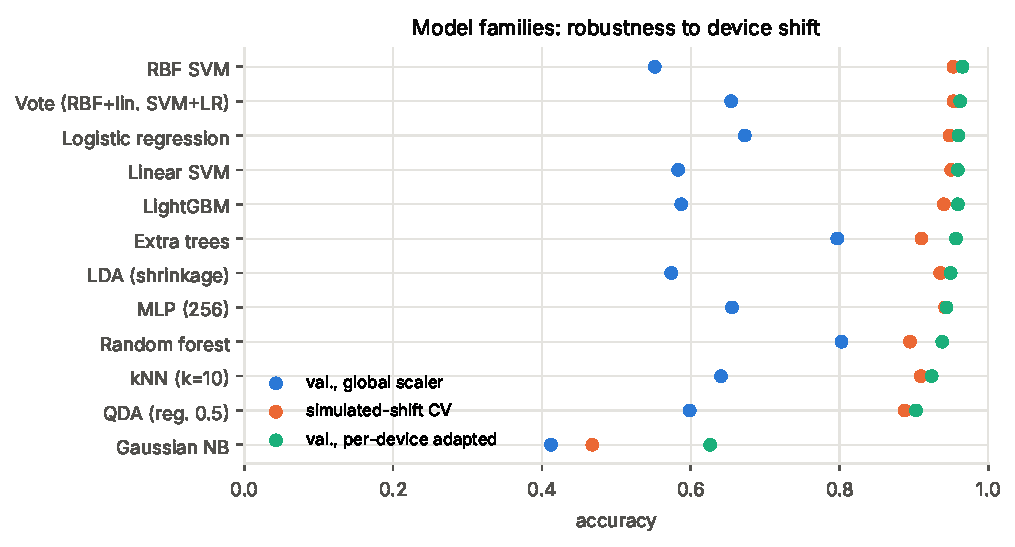
\includegraphics[width=\linewidth]{compare.pdf}
  \caption{Accuracy of each family: validation with a global scaler, simulated-shift CV, and
  validation with per-device adaptation.}
  \label{fig:compare}
\end{figure}

\subsection{Ablation}
\Cref{tab:ablation,fig:ablation} remove one step at a time from the shipped pipeline
(\AblShipped\,\%). Without per-device adaptation accuracy falls to \AblNoAdapt\,\%; without
feature selection to \AblNoSelect\,\%; without both to \AblNeither\,\%. Both steps are
necessary, and they interact: the noisy features hurt the RBF kernel far more once the
offsets are removed and they dominate the distances.

% GENERATED by `uv run poe experiments` — do not edit by hand.
\begin{table*}[t]
\centering
\small
\caption{Ablation with the shipped RBF SVM (accuracy \%). Per-device columns use the devices discovered on the validation set; variants without adaptation treat the set as one domain (--).}
\label{tab:ablation}
\begin{tabular}{lrrrr}
\toprule
Variant & Val. dev.\,0 & Val. dev.\,1 & Val. overall & Sim.-shift CV \\
\midrule
Shipped pipeline & 97.2 & 97.4 & 97.3 & 95.6 \\
No per-device adaptation (global scaler) & -- & -- & 75.9 & 18.4 \\
No feature selection (all 561) & 31.1 & 29.1 & 30.1 & 98.2 \\
No adaptation and no selection & -- & -- & 24.7 & 19.7 \\
No outlier clipping & 97.0 & 96.8 & 96.9 & 94.4 \\
Robust scaling (median/IQR) & 96.2 & 97.1 & 96.7 & 95.4 \\
Mutual-information top-315 & 81.4 & 80.6 & 81.0 & 96.2 \\
+ PCA (95\% variance) & 95.1 & 96.1 & 95.6 & 93.8 \\
+ LDA projection (5-D) & 95.6 & 96.2 & 95.9 & 58.2 \\
\bottomrule
\end{tabular}
\end{table*}


\begin{figure}[t]
  \centering
  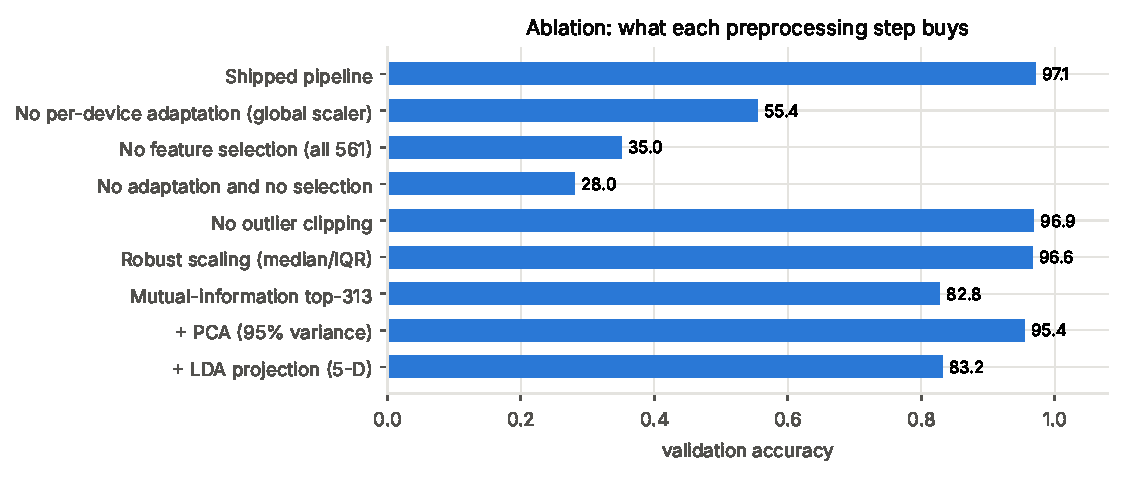
\includegraphics[width=\linewidth]{ablation.pdf}
  \caption{Ablation of the preprocessing (validation accuracy).}
  \label{fig:ablation}
\end{figure}

\subsection{Tuning}
\Cref{fig:tuning} shows the $C\times F_{\text{thr}}$ grid (range \GridMin--\GridMax\,\%). The
optimum is a broad plateau, so the chosen point ($C=\TunedC$, $F>\TunedF$, \TunedVal\,\%) is not
a sharp, validation-specific optimum.

\begin{figure}[t]
  \centering
  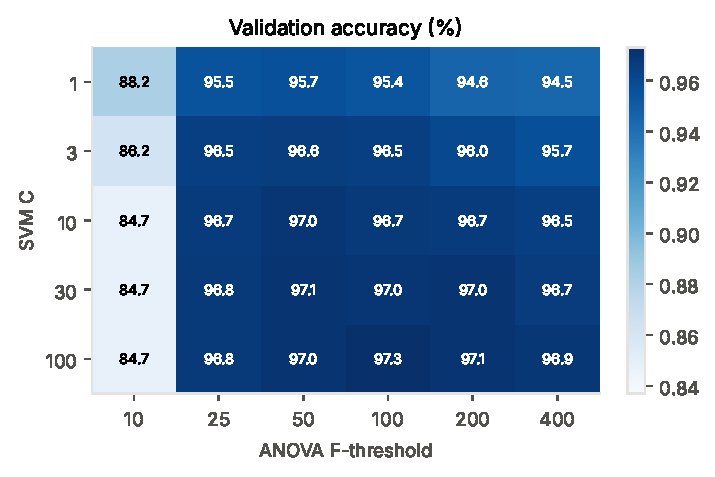
\includegraphics[width=0.85\linewidth]{tuning.pdf}
  \caption{Validation accuracy over SVM $C$ and ANOVA threshold.}
  \label{fig:tuning}
\end{figure}

\subsection{Robustness to controlled shifts}
\Cref{fig:robust} applies increasing synthetic shifts to a held-out 20\,\% of Device\_B.
Per-device adaptation makes accuracy invariant to calibration offsets and gains of any size,
while the global scaler collapses as soon as offsets exceed about one standard deviation.
Additive noise and outlier records degrade both variants. Adaptation does not remove noise,
which marks the method's limit.

\begin{figure}[t]
  \centering
  \begin{subfigure}{0.49\linewidth}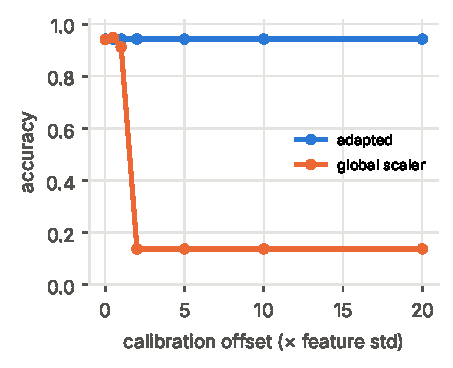
\includegraphics[width=\linewidth]{robustness_offset.pdf}\end{subfigure}
  \begin{subfigure}{0.49\linewidth}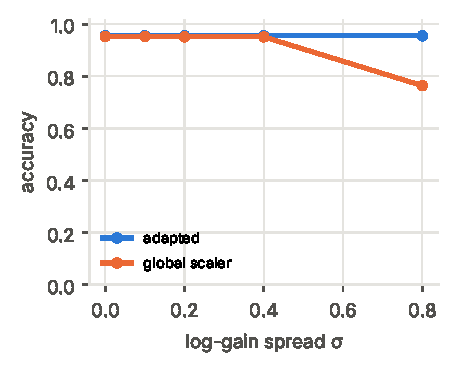
\includegraphics[width=\linewidth]{robustness_gain_sigma.pdf}\end{subfigure}
  \begin{subfigure}{0.49\linewidth}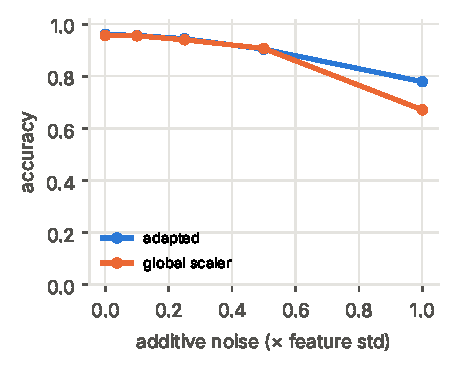
\includegraphics[width=\linewidth]{robustness_noise.pdf}\end{subfigure}
  \begin{subfigure}{0.49\linewidth}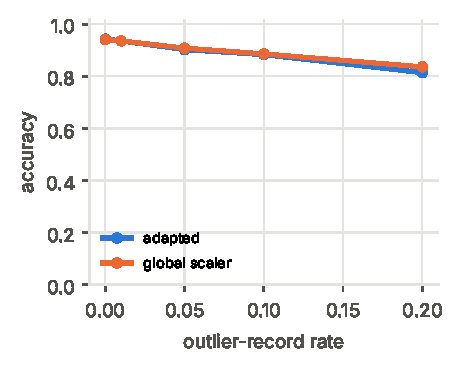
\includegraphics[width=\linewidth]{robustness_outlier_fraction.pdf}\end{subfigure}
  \caption{Accuracy under controlled synthetic device shifts: adapted vs.\ global scaler.}
  \label{fig:robust}
\end{figure}

\subsection{Final system and error analysis}
Through the exact \texttt{infer.py} code path, the shipped model reaches \FinalAcc\,\% accuracy
(macro-F1 \FinalMacroF\,\%) on the validation set: \FinalDevZero\,\% and \FinalDevOne\,\% on the
two discovered devices (\cref{tab:per_class,fig:confusion}). The dominant failure mode is
Sitting~$\leftrightarrow$~Standing (\SitStand{} of the errors): both are static, upright
postures with nearly identical inertial signatures, the classic confusion on this feature
set~\cite{anguita2013}. Dynamic classes are rarely confused with static ones, and Laying is
almost always correct thanks to its distinct gravity orientation.

Timing: mean \FinalMeanMs\,ms and 95th percentile \FinalPNinetyFiveMs\,ms per sample as written to
\texttt{time.txt}, \FinalTotalS\,s in total for \NVal{} samples including the amortized
adaptation (\cref{fig:timing}).

% GENERATED by `uv run poe experiments` — do not edit by hand.
\begin{table}[t]
\centering
\small
\caption{Shipped model on the validation set, through the real \texttt{infer.py} path (\%).}
\label{tab:per_class}
\begin{tabular}{lrrrr}
\toprule
Activity & Precision & Recall & F1 & Support \\
\midrule
0 Walking & 99.2 & 99.2 & 99.2 & 526 \\
1 Walking Upstairs & 99.6 & 99.0 & 99.3 & 482 \\
2 Walking Downstairs & 98.8 & 99.5 & 99.1 & 402 \\
3 Sitting & 91.9 & 94.4 & 93.1 & 517 \\
4 Standing & 94.9 & 92.6 & 93.7 & 582 \\
5 Laying & 100.0 & 100.0 & 100.0 & 581 \\
\bottomrule
\end{tabular}
\end{table}


\begin{figure}[t]
  \centering
  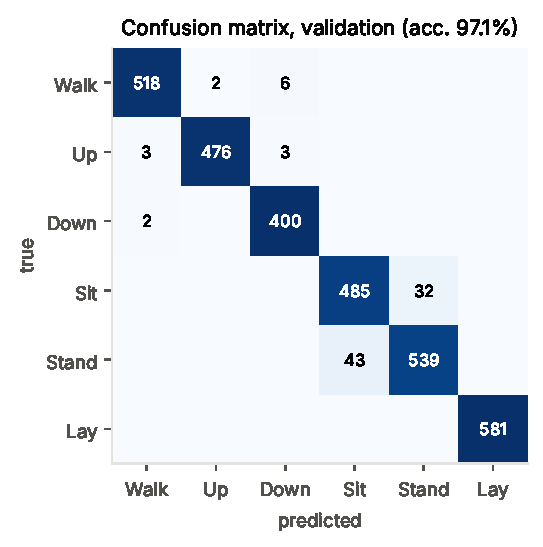
\includegraphics[width=0.8\linewidth]{confusion.pdf}
  \caption{Confusion matrix of the shipped model on the validation set (counts; colour = row-normalized).}
  \label{fig:confusion}
\end{figure}

\begin{figure}[t]
  \centering
  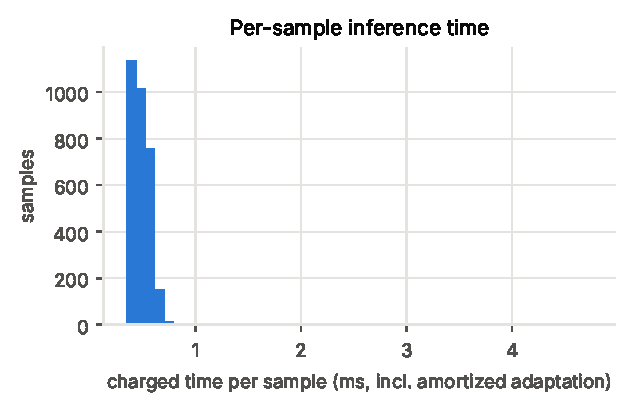
\includegraphics[width=0.8\linewidth]{timing.pdf}
  \caption{Per-sample time charged in \texttt{time.txt}.}
  \label{fig:timing}
\end{figure}
